% CHAPITRE 2
% SUIVI VARIABILITE SPATIALE

\chapter{Sites d'études et méthodologies employées}
\newpage

\section{Présentation des sites d'études}

L'ensemble des sites d'études sont regroupés au sein d'un service d'observation

\subsection{La Guette}

La tourbière de La Guette est situé à Neuvy-sur-Barangeon, en Sologne, dans le département du Cher.
Le site s'étend sur une surface d'une vingtaine d'hectare avec une géométrie relativement allongée.
Avec une conductivité généralement inférieur à 80 uS/m2 et un pH compris entre 4 et 5 elle se classe parmis les "transitionnal poor fen"
Les datations effectuées sur le site permettent de dire que la tourbière est agée de 5 à 6000 ans.
Dans les années 19XX la construction d'une route coupe la tourbière dans sa partie sud.
En 2008 le récurage du fossé de drainage bordant la route semble entrainer une augmentation significative des pertes d'eau du système.

Des travaux (SOURCE, Émelie) d'analyse de photos aériennes ont ainsi montré une progression importante du boisement (principalement des pins (pinus Sylvestris) et des bouleau (Betula sp.). Des herbacées envahissent également le site avec une forte présence de la molinie (Molinia caerulea)

Sont présente sur le site un certain nombre d'espèces caractéristiques des tourbières comme les sphaignes (principalement Sphagnum cuspidatum et Sphagnum rubellum) et Eriophorum augustifolium.

\begin{figure}
\centering
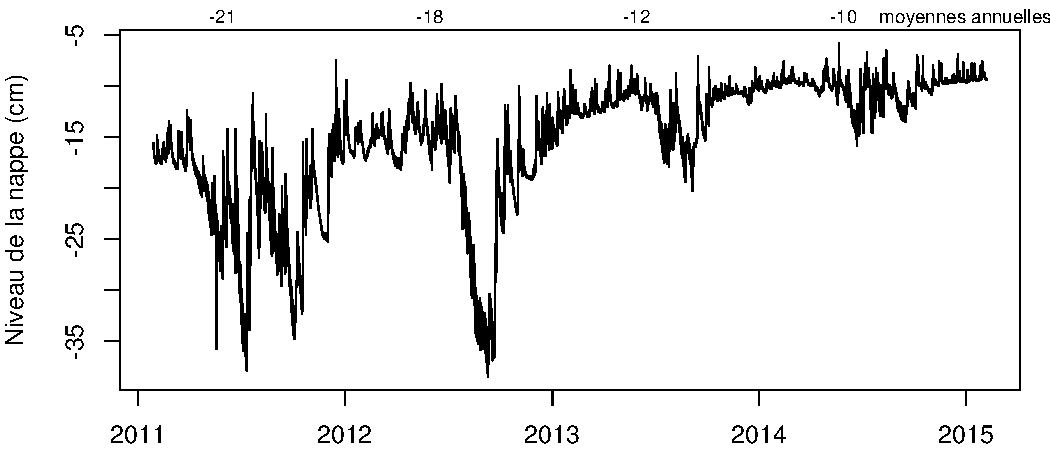
\includegraphics[width=\textwidth]{WTL}
\caption{Évolution du niveau de la nappe, en cm par rapport à la surface, des années 2011 à 2014}
\label{fig:WTL}
\end{figure}

\begin{figure}
\centering
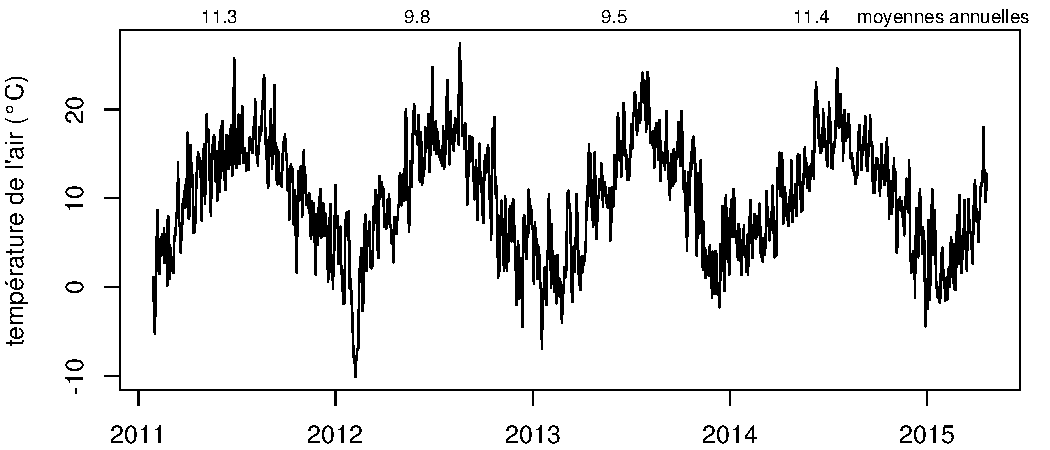
\includegraphics[width=\textwidth]{tair}
\caption{Évolution de la température de l'air (en \textdegree C) des années 2011 à 2014}
\label{fig:tair}
\end{figure}

\begin{figure}
\centering
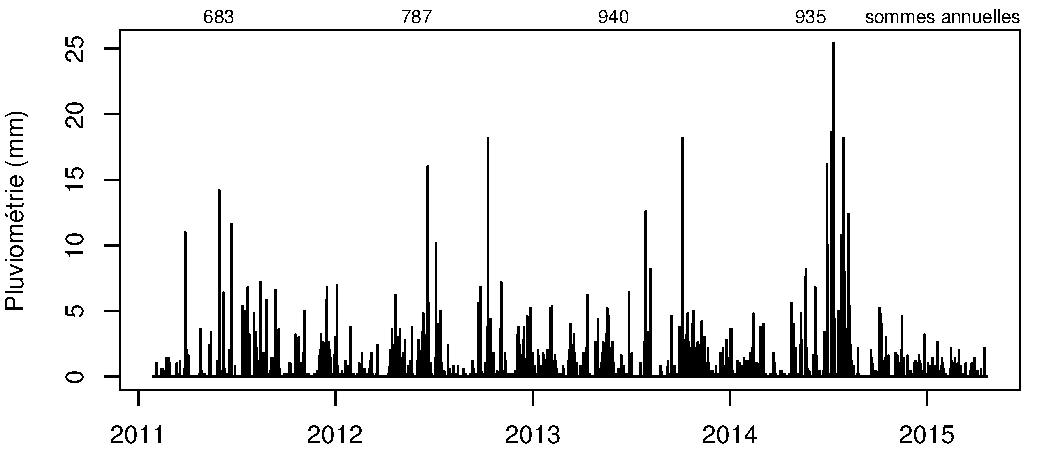
\includegraphics[width=\textwidth]{pluvio}
\caption{Évolution du niveau de la pluviométrie, en \si{\mm}, des années 2011 à 2014}
\label{fig:pluvio}
\end{figure}


\subsection{Frasne}

\subsection{Landemarais}

\subsection{Bernadouze}


Au sein de ses sites de nombreuses mesures ont été effectuée et notamment des mesures de flux de GES à la fois concernant le CO2 et le CH4. La méthodologie étant transverse à de nombreuses expérimentations il convient de l'expliquer au préalable.

\section{Mesures de flux}
\label{sec:clsd_chbr_method}

Il existe de nombreuses façon de mesurer des flux de gaz. 
Des méthodes globale comme les tour à flux utilisant des méthodes d'Eddy Covariance. 
Des méthodes plus locale, les chambres d'accumulation de gaz qui peuvent être statique ou dynamique, selon que la sonde mesurant le gaz soit directement dans la chambre ou que le gaz soit apportée à cette dernière via un système de pompe. Elles peuvent être ouverte ou fermée.

La méthode de mesure retenue pour ces travaux est l'utilisation de chambre statique fermée, permettant une mesure locale et directe des flux.
Pour cela des embases sont placées sur le terrain. Il s'agit de cylindre de PVC d'une dizaine de cm, percés dans leur partie basse afin de minimiser les impacts sur les flux d'eau et sur de développement racinaire et enfoncé dans le sol.
Les embases sont généralement posée 12h avant toute mesure afin de ne pas mesurer de dégagement gazeux liés à l'installation.

Que mesure-t-on ?
Le plus souvent 2 mesures consécutives sont effectuées la première avec une chambre transparente permettant d'accéder à la NEE et l'autre avec une chambre recouverte d'un isolant permettant de bloquer la lumière et permettant de mesurer les respirations. (pourquoi les respirations?)

De nombreux écueils peuvent rendre une mesure inexploitable. D'abord le placement de la chambre, cela peut sembler trivial mais positionner la chambre au milieu d'herbacées et de bruyère n'est pas tourjours évident. Plus anectdotiquement des sphaignes gelées, recouvrant les bords de l'embase rendent la pose de la chambre difficile voire impossible. Selon l'heure de la journée des gradients de concentrations peuvent être présent et augmenter localement les concentrations de CO2 de façon importante allant jusqu'à saturer la sonde.

QUESTIONS :

*Taille des embases ? Effets de bord ?
*Perturbation du milieu ? (Mesure de végétation, pose de la chambre, mesure pièzo...)
*Impact de la strate arborée ?
*Validité des profils de température ?
Méthode de Chambre fermée (Biais ?)

Améliorations ? \todo[inline]{Lister les amélioration à faire ou non}


\section{Facteurs contrôlants et suivi des flux}
Afin de déterminer l'impact de facteurs contrôlants sur ces flux, mesurer les flux ne suffit pas il faut également mesurer les variables environnementales dont on pense qu'elles seront des facteurs contrôlants important. Le nombre de ces variables et la méthodologie employée pour les mesurer étant différente selon l'expérimentation ils seront détaillés au fil des besoins par la suite.

\section{Protocole d'estimation de la végétation}


\section*{Bilan des mesures effectuées ?}